\documentclass[10pt,a4paper]{article}
\usepackage[margin=2.2cm]{geometry}
\usepackage{fontspec}
\usepackage{kotex}
\setmainfont{Apple SD Gothic Neo}
\setsansfont{Apple SD Gothic Neo}
\usepackage{amsmath,amssymb}
\usepackage{graphicx}
\usepackage{booktabs}
\usepackage{caption}
\usepackage[dvipsnames]{xcolor}
\usepackage[colorlinks=true,linkcolor=MidnightBlue,citecolor=MidnightBlue,
            urlcolor=MidnightBlue]{hyperref}
\usepackage{titlesec}
\titleformat{\section}{\large\bfseries}{\thesection}{0.6em}{}
\titleformat{\subsection}{\normalsize\bfseries}{\thesubsection}{0.5em}{}
\captionsetup{font=small,labelfont=bf}
\setlength{\parskip}{0.35em}
\setlength{\parindent}{0pt}

\usepackage{mdframed}
\newmdenv[linewidth=0.4pt,linecolor=gray!60,backgroundcolor=gray!5,
          innertopmargin=6pt,innerbottommargin=6pt,skipabove=8pt,skipbelow=8pt]{claimbox}
\newcommand{\claim}[2]{\begin{claimbox}\textbf{주장.} #1\par\smallskip
  \textcolor{gray!70}{\textbf{반증 조건.} #2}\end{claimbox}}

\title{\bfseries 교집합이 비어 있다\\[2pt]
\large 장소와 방문객을 다 가진 프로젝트가 $0$건이었다 --- 그래서 갈래 하나를 버린다}
\author{월드모델 실험실 · 노트 772 · 773}
\date{2026-08-07}
\begin{document}\maketitle

\section{한 줄}

논문 $152$ 가 T2 를 쉼으로 내리고 다시 열 조건을 값으로 적었다 --- \textbf{시군구 고정
가능한 방문객 라벨 $2{,}028$행}(현재 $62$행). 그리고 \emph{``그 행수는 채굴이 아니라
레코드 생성으로 와야 한다''}를 적었다.

\textbf{그 길을 셌다. 교집합이 $0$ 건이다.} 장소 링크가 있는 프로젝트 $21$개, 방문객이
있는 프로젝트 $7$개, \textbf{둘 다 가진 것 $0$개.} 방문객 행 $48$개의
\texttt{venue\_id} 는 \textbf{전부 NULL} 이다.

\textbf{그래서 팝업 방문객 갈래를 파운데이션 목적에서 내린다.} 상시 지시가
\emph{``팝업은 여러 도메인 중 하나일 뿐이고 안 되면 버린다''}이고, \textbf{버릴 근거가
셋 모였다.}

\section{읽기 전용으로만 셌다}

\textbf{제약 준수}: BQ 는 \texttt{INFORMATION\_SCHEMA} 메타조회와 \texttt{SELECT} 만 ·
\textbf{아무것도 쓰지 않았다.}

\begin{center}
\begin{tabular}{lrl}
\toprule
표 & 행 & \\
\midrule
\texttt{core.engagement} & $579$ & $2023$-$01$-$01 \sim 2026$-$12$-$18$ · 갈래 코드 NULL $0$건 \\
\texttt{core.engagement\_venue} & $21$ & $21$ engagement · $19$ venue \\
\texttt{core.popup\_visitor\_daily} & $48$ & \textbf{$7$ engagement} · $2026$-$06$-$12 \sim 08$-$04$ · 합 $38{,}528$ \\
& & \textbf{\texttt{venue\_id} 가 붙은 행 $\mathbf{0}$개} \\
\midrule
\textbf{장소 $\cap$ 방문객} & $\mathbf{0}$ & 둘 중 하나라도 가진 것 $28$건 \\
\bottomrule
\end{tabular}
\end{center}

T7 자신의 문턱은 \emph{``$20$건 이상이면 레코드 생성이 채굴보다 값이 크다''}였다.
\textbf{$0$ 건이다.}

\begin{figure}[t]\centering
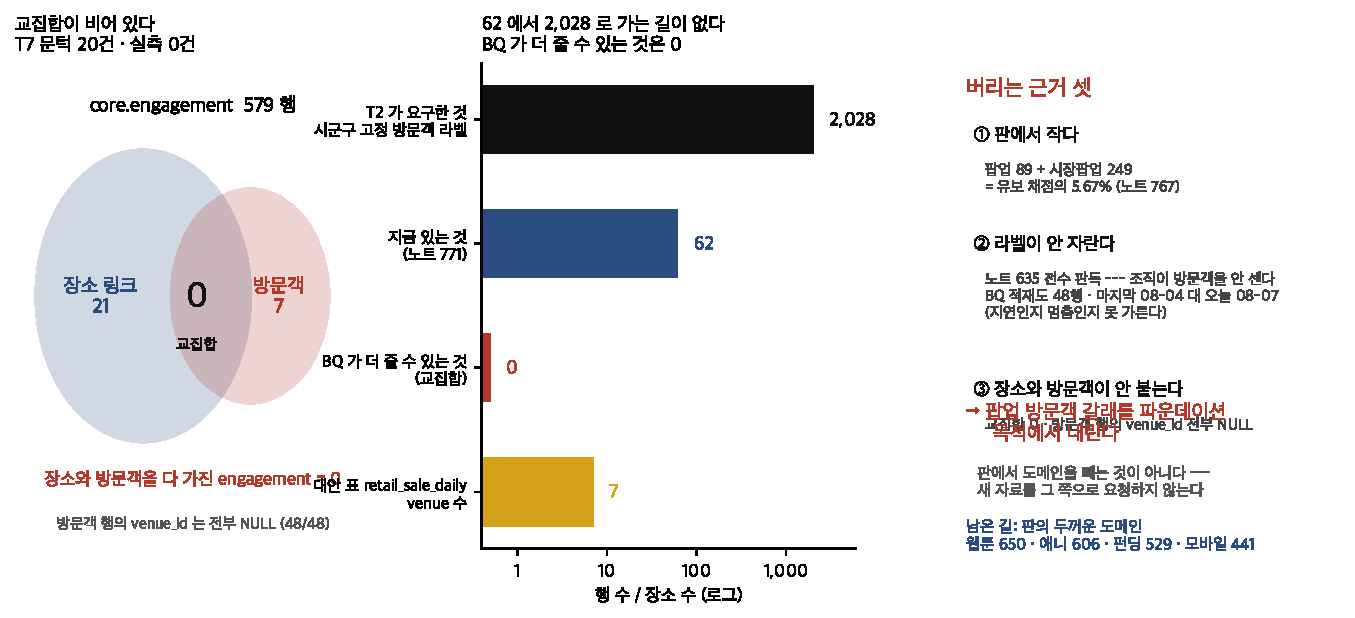
\includegraphics[width=0.99\textwidth]{figs/emptyjoin.pdf}
\caption{왼쪽: \textbf{교집합이 비어 있다.} 가운데: \textbf{$62$에서 $2{,}028$로 가는
길이 없다} --- BQ 가 더 줄 수 있는 것은 $0$이고 대안 표는 장소가 $7$개다. 오른쪽:
\textbf{버리는 근거 셋.}}
\end{figure}

\subsection*{방문객 $7$건이 새 자료가 아니다}

그 $7$ 프로젝트는 \textbf{RCPU$2631 \cdot 2636 \cdot 2637 \cdot 2639 \cdot 2640 \cdot
2641 \cdot 2642$} 다. \textbf{전부 이미 감사의 ``승인 대기'' 목록에 있는 라벨
후보}다(노트 $636 \cdot 673$).

\claim{\textbf{``레코드 생성 경로''가 새 행을 안 만든다.} BQ 가 준 것은 새 자료가
아니라 \textbf{이미 사람 확인을 기다리는 여섯 건}이다. 그러므로 그 경로는
$62 \to 2{,}028$ 의 $33$배를 채울 수 없다.}
{적재가 앞으로 쌓일 수 있다 --- 노트 $636$ 이 \emph{``앞으로만 쌓이므로 채굴보다 배선이
값이 크다''}를 적었다. \textbf{그 기대를 지금 반증하지는 못한다} --- 마지막 방문일이
$08$-$04$ 이고 오늘이 $08$-$07$ 이라 사흘 공백이지만 \textbf{지연인지 멈춤인지 이
시점에 못 가른다.} 관측 창을 적어 둔다: \textbf{첫 적재(노트 $636$ · $08$-$05$) 이후
이틀 동안 $48$행 그대로}다.}

\subsection*{맞추기는 못 했다 --- 틀림 조건이 발동했다}

우리 레코드 $380$건에 \textbf{engagement 식별자가 없다}(\texttt{engagement\_id} ·
\texttt{engagement\_code} 필드 $0$건 · \texttt{PJ} 코드 $4$건뿐 · \texttt{provenance} 는
\texttt{extracted\_at/by} · \texttt{notes} · \texttt{reviewed\_by} 만).

\textbf{그래서 ``레코드 없는 engagement''를 셀 수 없다.} 사전등록 틀림 조건 ②가
그 경우를 미리 적었고 --- \emph{``맞추기를 포기하고 전체 대 우리 것만 적는다''} ---
\textbf{$579$ 대 $380$ 만 적는다.} \textbf{모르는 것을 아는 것처럼 쓰지 않는다.}

\section{대안 결과 변수도 막혔다}

노트 $688$ 이 \emph{``$L$ 을 다른 결과 변수(웨이팅 · 체류 · 재방문)로 옮겨야 한다''}를
적었다. 방문객이 아닌 것을 찾았다.

\begin{center}
\begin{tabular}{lrl}
\toprule
\texttt{core.occupancy} & $0$행 & \\
\texttt{core.retail\_sale\_daily} & $6{,}636$행 & $2025$-$03$-$24 \sim 2026$-$06$-$29$ ·
brand $187$ · venue$\times$날 $1{,}104$ \\
& & \textbf{그런데 venue 가 $\mathbf{7}$개다} \\
\bottomrule
\end{tabular}
\end{center}

\claim{\textbf{$6{,}636$행이 있어도 장소가 $7$개면 T2 의 요구를 못 채운다.} 논문 $152$ 가
요구한 것은 \emph{``$2{,}028$행 \textbf{그리고 동네가 골고루}''}였고 \textbf{$7$ 장소는
그 반대}다. 행수가 아니라 \textbf{클러스터 수}가 판정력을 정한다는 것이 논문 $152$ 의
결론이었다.}
{매출을 \emph{다른 물음}에 쓸 수는 있다 --- 예컨대 ``같은 장소에서 브랜드가 바뀌면 매출이
어떻게 바뀌나''는 $7$ 장소 $\times$ $187$ 브랜드로 물을 수 있고, 그것은 장소 고정
설계다. \textbf{그러나 그것은 $L(g,\text{event})$ 가 아니다} --- $g$ 는 동네 상태이고
장소 $7$개로는 동네 변동을 못 본다.}

\section{그래서 갈래 하나를 버린다}

\begin{center}
\begin{tabular}{ll}
\toprule
\textbf{① 판에서 작다} & 팝업 $89$ $+$ 시장팝업 $249$ $=$ 유보 채점의 $\mathbf{5.67\%}$(논문 $150$) \\
\textbf{② 라벨이 안 자란다} & 노트 $635$ 가 이미지 PDF $77$건 전수 판독으로 \\
& \textbf{``조직이 방문객을 안 센다''}를 확정 · BQ 적재도 $48$행 \\
\textbf{③ 장소와 방문객이 안 붙는다} & 교집합 $0$ · 방문객 행의 \texttt{venue\_id} 전부 NULL \\
\bottomrule
\end{tabular}
\end{center}

\claim{\textbf{팝업 방문객을 키워 파운데이션에 기여시키는 갈래를 내린다.} 상시 지시가
\emph{``안 되면 버린다''}이고 근거가 셋이다. \textbf{판에서 팝업 도메인을 빼는 것이
아니다} --- 빼면 판이 바뀌므로 안 뺀다. \textbf{새 자료를 그 쪽으로 요청하지 않는다는
뜻이다.}}
{②가 완전히 확정된 것은 아니다 --- \textbf{적재가 앞으로 쌓이면 ②가 약해진다.} 그러면
버린 결정을 되돌려야 한다. \textbf{되돌릴 조건을 값으로 적는다}: \texttt{popup\_visitor\_daily}
가 \textbf{$500$행 이상이 되고 그중 $100$행 이상에 \texttt{venue\_id} 가 붙으면} 다시
센다. 지금은 $48$행 · $0$개다.}

\subsection*{남은 길 --- 판의 두꺼운 도메인}

\begin{center}
웹툰 $650$ · 애니 $606$ · 펀딩 $529$ · 모바일 $441$ · 세계애니 $300$ · 만화 $258$\\
(유보 채점 기준. 팝업 $65$ · 시장팝업 $126$)
\end{center}

\claim{\textbf{T7 의 다음 물음이 바뀐다} --- ``팝업 라벨을 어떻게 더 캐나''에서
\textbf{``판의 두꺼운 도메인 원천에 아직 안 쓰는 열이 있나''}로. 결정 규칙을 값으로
적었다: 도메인마다 원천 열 목록과 판이 쓰는 특징 목록을 맞춰 \textbf{안 쓰는 열 중 시간
게이트를 통과하는 것이 도메인당 $3$개 이상}이면 후보 축이 남아 있고, \textbf{미만이면
원천이 마른 것}이라 외부 API 가 유일한 길이다.}
{그 셈도 열 이름으로 세는 것이라 \textbf{자유 텍스트에 숨은 정보를 놓친다}(논문 $150$
에서 같은 한계를 적었다). 그리고 \textbf{``안 쓰는 열''이 많아도 신호가 없을 수
있다} --- 논문 $146$ 이 ``차원 비용'' 변명을 죽였으므로 넣어 보는 것은 싸다($1$열
$\approx 0.006$). \textbf{즉 이 셈은 희망의 상한이고 결론이 아니다.}}

\end{document}
